\label{chapter-scenario-template}
\textbf{Created by:} Perawit Charoenwut \\
\textbf{Modified by:}

\subsection*{Scenario Objective}
This scenario illustrates how to represent a complete company structure with manufacturing and business divisions using the IOF core ontology. It focuses on:
\begin{itemize}
    \item Showing how business and manufacturing units coexist within one company
    \item Distinguishing between business and manufacturing activities
    \item Capturing different organizational roles and functions
\end{itemize}

\subsection*{General Pattern Description}
A company can contain both business organizations and manufacturers as part of its structure.
An Organization can simultaneously be:
\begin{enumerate}
    \item A BusinessOrganization that has a BusinessFunction, which is realized through a SellingBusinessProcess that sells the MaterialProduct
    \item A Manufacturer that has a ManufacturerRole, which is realized through a ProductProductionProcess and  has the MaterialProduct as its output.
\end{enumerate}

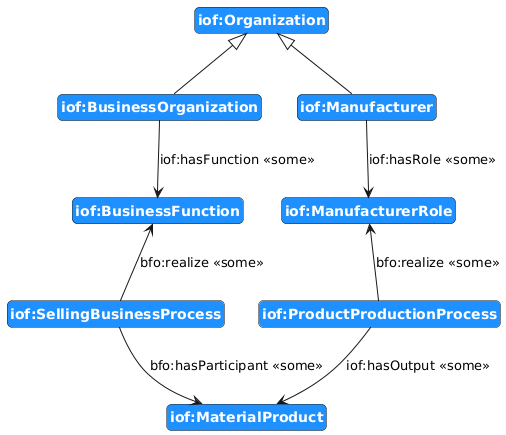
\includegraphics[scale=0.6]{scenarios/different-type-organizations/image/different-type-organizations-schema}

\subsection*{Use Case: }

This use case demonstrates how a company like GE operates as both a manufacturer and a business organization using the same material products.

\subsubsection*{Use-Case Pattern Description}
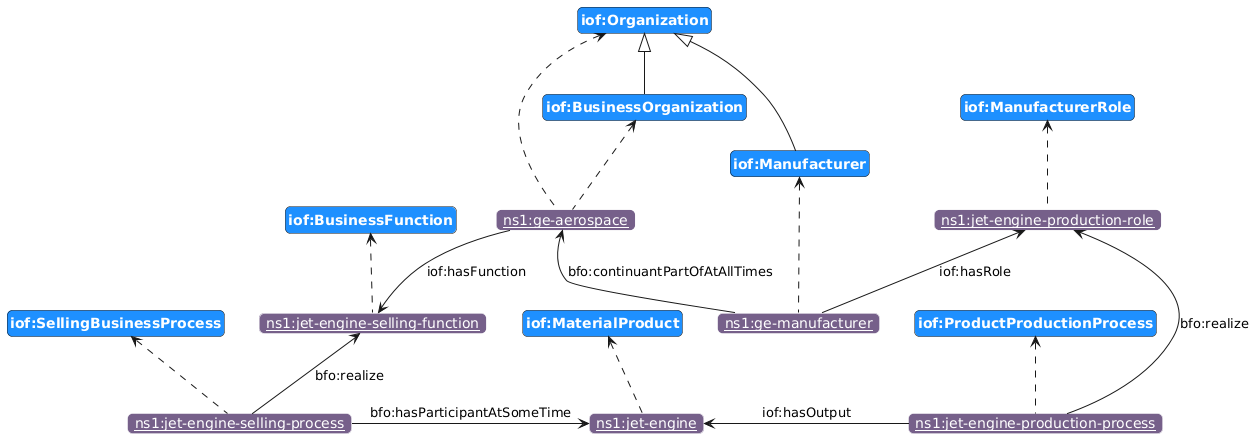
\includegraphics[scale=0.35]{scenarios/different-type-organizations/image/different-type-organizations}

GE Aerospace (\texttt{ns1:ge-aerospace}) operates as both an organization (\texttt{iof:Organization}) and a business organization (\texttt{iof:BusinessOrganization}) with respect to jet engines (\texttt{ns1:jet-engine}). Through its manufacturing division (\texttt{ns1:ge-manufacturer}), which is \texttt{bfo:continuantPartOfAtAllTimes} of GE Aerospace, it bears a manufacturer role (\texttt{ns1:jet-engine-production-role}) which is \texttt{bfo:realize} through a production process (\texttt{ns1:jet-engine-production-process}), producing jet engines as \texttt{iof:hasOutput}. The organization also has a business function (\texttt{ns1:jet-engine-selling-function}) which is \texttt{bfo:realize} through a selling process (\texttt{ns1:jet-engine-selling-process}), where the same jet engines are sold (\texttt{bfo:hasParticipantAtSomeTime}) in the selling process.
\subsubsection*{Use-Case Example Data}


\begin{table}[h]
% \caption{}
\label{tab:organization-structure}
% \resizebox{\columnwidth}{!}{%
\begin{tabular}{|l|l|}
\hline
Entity & Function/Role \\ \hline
GE Aerospace & Sells products and has Manufacturer \\
GE Manufacturer & Manufactures products \\
Jet engine & Product \\
\hline
\end{tabular}%
% }
\end{table}


\subsubsection*{Data Mapping}
\begin{verbatim}
INSERT DATA {
    ns1:ge-aerospace a iof:Organization, iof:BusinessOrganization;
        iof:hasFunction ns1:jet-engine-selling-function.
    
    ns1:ge-manufacturer a iof:Manufacturer;
        bfo:continuantPartOfAtAllTimes ns1:ge-aerospace;
        iof:hasRole ns1:jet-engine-production-role.
    
    ns1:jet-engine-selling-function a iof:BusinessFunction.
    ns1:jet-engine-selling-process a iof:SellingBusinessProcess;
        bfo:realize ns1:jet-engine-selling-function;
        bfo:hasParticipantAtSomeTime ns1:jet-engine.
    
    ns1:jet-engine-production-role a iof:ManufacturerRole.
    ns1:jet-engine-production-process a iof:ProductProductionProcess;
        bfo:realize ns1:jet-engine-production-role;
        iof:hasOutput ns1:jet-engine.
    
    ns1:jet-engine a iof:MaterialProduct.
    
    iof:BusinessOrganization rdfs:subClassOf iof:Organization.
    iof:Manufacturer rdfs:subClassOf iof:Organization.
}
\end{verbatim}



\subsubsection*{Data Validation}
\begin{verbatim}
#Shape for iof:BusinessOrganization
ns1:BusinessOrganizationShape a sh:NodeShape ;
    sh:targetClass iof:BusinessOrganization ;
    sh:property [
        sh:path iof:hasFunction ;
        sh:class iof:BusinessFunction ;
        sh:minCount 1 ;
    ] ;
    sh:property [
        sh:path rdfs:subClassOf ;
        sh:hasValue iof:Organization ;
    ] .

#Shape for Manufacturer
ns1:ManufacturerShape a sh:NodeShape ;
    sh:targetClass iof:Manufacturer ;
    sh:property [
        sh:path iof:hasRole ;
        sh:class iof:ManufacturerRole ;
        sh:minCount 1 ;
    ] ;
    sh:property [
        sh:path rdfs:subClassOf ;
        sh:hasValue iof:Organization ;
    ] .

# Shape for SellingBusinessProcess
ns1:SellingBusinessProcessShape a sh:NodeShape ;
    sh:targetClass iof:SellingBusinessProcess ;
    sh:property [
        sh:path bfo:realize ;
        sh:class iof:BusinessFunction ;
        sh:minCount 1 ;
    ] ;
    sh:property [
        sh:path bfo:hasParticipantAtSomeTime ;
        sh:class iof:MaterialProduct ;
        sh:minCount 1 ;
    ] .

# Shape for ProductProductionProcess
ns1:ProductProductionProcessShape a sh:NodeShape ;
    sh:targetClass iof:ProductProductionProcess ;
    sh:property [
        sh:path bfo:realize ;
        sh:class iof:ManufacturerRole ;
        sh:minCount 1 ;xf
    ] ;
    sh:property [
        sh:path iof:hasOutput ;
        sh:class iof:MaterialProduct ;
        sh:minCount 1 ;
    ] .
\end{verbatim}
